\documentclass[a4paper,12pt]{article}   % papír A4, písmo 12 bodu
\usepackage[utf8x]{inputenc}            %kodovaní UTF-8
\usepackage{ucs}                        %kodovani unicode
\usepackage[czech]{babel}               %podpora cestiny
\usepackage[T1]{fontenc}                %pouzij variantu pisma T1 (hacky, carky)
\usepackage[left=2.5cm,right=1.5cm,top=2.5cm,bottom=2.5cm]{geometry} %okraje stranky
\usepackage{amsmath,amsfonts,amssymb}   %podpora matematiky
\usepackage{gensymb,marvosym}           %symboly celsius (\celsius) apod.
%\usepackage{mathptmx}                   %font Times New Roman s~podporou matematiky
\usepackage{times}                      %font Times New Roman (matematika pismem Computer Modern) 
\usepackage{parskip}                    %mezera mezi odstavci
%\usepackage[document]{ragged2e}         %text zarovany vlevo
\usepackage[none]{hyphenat} \sloppy     %slova nedelit a~nepretekat
\usepackage{titlesec}
\setcounter{secnumdepth}{4}
\clubpenalty 10000                      %kontrolovat sirotky
\widowpenalty 10000                     %kontrolovat vdovy
\usepackage{setspace} \onehalfspacing   %podpora pro zmenu radkovani + radkovani 1,5
\usepackage{enumerate}                  %podpora pro zmenu cislovani
\usepackage{fancyhdr}                   %vlastni zahlavi a~zapati
\usepackage{graphicx}                   %podpora grafiky
\graphicspath{{materialy/}}                   %vychozi adresar s~obrazky
\usepackage{caption}                    %popisky
\usepackage{subcaption}                 %podpopisky
\usepackage{siunitx}
\usepackage{MnSymbol,wasysym}
\usepackage[shortlabels]{enumitem}
\usepackage{amsmath}
\usepackage{lastpage}                   %zjištění poslední stránky \pageref{LastPage}
\usepackage{float}                      
\usepackage{url}
\usepackage[unicode]{hyperref}          %klikaci odkazy v~textu
\usepackage{mhchem}
\usepackage{multirow}

\usepackage{halloweenmath}


\titleclass{\subsubsubsection}{straight}[\subsection]
\newcounter{subsubsubsection}[subsubsection]
\renewcommand\thesubsubsubsection{\thesubsubsection.\arabic{subsubsubsection}}
\renewcommand\theparagraph{\thesubsubsubsection.\arabic{paragraph}} % optional, useful if paragraphs are to be numbered


%------------------------ čtvrtá a~pátá úroveň nadpisu ---------------------------

\titleformat{\subsubsubsection}
  {\normalfont\normalsize\bfseries}{\thesubsubsubsection}{1em}{}
\titlespacing*{\subsubsubsection}
{0pt}{3.25ex plus 1ex minus .2ex}{1.5ex plus .2ex}

\makeatletter

\renewcommand\paragraph{\@startsection{paragraph}{5}{\z@}%
  {3.25ex \@plus1ex \@minus.2ex}%
  {-1em}%
  {\normalfont\normalsize\bfseries}}
\renewcommand\subparagraph{\@startsection{subparagraph}{6}{\parindent}%
  {3.25ex \@plus1ex \@minus .2ex}%
  {-1em}%
  {\normalfont\normalsize\bfseries}}
\def\toclevel@subsubsubsection{4}
\def\toclevel@paragraph{5}
\def\toclevel@paragraph{6}
\def\l@subsubsubsection{\@dottedtocline{4}{7em}{4em}}
\def\l@paragraph{\@dottedtocline{5}{10em}{5em}}
\def\l@subparagraph{\@dottedtocline{6}{14em}{6em}}
\makeatother

\setcounter{secnumdepth}{4}
\setcounter{tocdepth}{4}


\setlist[enumerate]{itemsep=0mm}
%_____________________________|___________________________|_____________________________%
%                             |                           |                             %
%-----------------------------| ZDE VYPLNIT UDAJE O PRACI |-----------------------------%
%_____________________________|___________________________|_____________________________%
%                             

\newcommand{\nazev}{MĚŘENÍ KMITOČTU A DOBY PERIODY ČÍTAČEM}                                                        %
\newcommand{\jmeno}{Jakub Dvořák}                                                     %
\newcommand{\datum}{27.10.2020}                                                              %
%---------------------------------------------------------------------------------------%


%-----------------------------| POUŽITÁ MAKRA |-----------------------------%

%\newcommand{\zkratka}{ve výsledku se mi napíše tenhle text}
%\newcommand{}{}
%\newcommand{}{}
%\newcommand{}{}
\newcommand{\tsub}[1]{$_\textrm{#1}$}
\newcommand{\texp}[1]{$^\textrm{#1}$}
\newcommand{\tohm}{$\Omega$}
\newcommand{\tmu}{$\mu$}


%_______________________________________________________________________________________%
%_______________________________________________________________________________________%


%----------------------------------- KONEC PREAMBULE -----------------------------------%






%-------------------------------------- DOKUMENT --------------------------------------%
%______________________________________________________________________________________%
\begin{document} %%%%%%%%%%%%%%%%%%%%%%%%%%%%%%%%%%%%%%%%%%%%%%%%%%%%%%%%%%%%%%%%%%%%%%%

\setcounter{page}{0} %cislo strany
\pagestyle{empty} %stranku necislovat

%prostredi pro grafy a~schemata \begin{graf} \begin{schema}
\newfloat{schema}{htbp}{schema}\floatname{schema}{Schéma}
\newfloat{graf}{htbp}{graf}\floatname{graf}{Graf}

\begin{titlepage}
    \begin{center}
        \vspace*{1cm}
            
        \Huge
        \textbf{\nazev}
            
        \vspace{0.5cm}
        \LARGE
            
        \vspace{1.5cm}
            
        \textbf{\jmeno}
            
        \vfill
            
        \vspace{0.8cm}
            
        \Large
            
        \datum\\
        \vspace*{.5cm}
        
\includegraphics[width=.4\textwidth]{logo-cvut-fee.png}\\
    \end{center}
\end{titlepage}

% --- definice zapati a~cislovani ---
\newpage 
\pagestyle{fancy}                                       %vlastni zahlavi/zapati
\renewcommand{\headrulewidth}{0pt}                      %bez linky v~zahlavi
\renewcommand{\footrulewidth}{.5pt}                    %linka v~zapati - optional
\lhead{}       \chead{} \rhead{\nazev}                        %pole zahlavi (prazdna)
\lfoot{\jmeno} \cfoot{} \rfoot{\thepage}   %pole zapati


%------------------------------------ VLASTNÍ TEXT ------------------------------------%



\section{Úkol měření}
\label{chap:zadani}
\begin{enumerate}
    \item Nakreslete blokové schéma čítače v~obou režimech činnosti.
    \item Zkontrolujte správnost stupnice nízkofrekvenčního generátoru:
    \begin{enumerate}[label=\alph*)]
        \item čítačem v~režimu \textbf{měření frekvence při různých dobách měření},
        \item čítačem v~režimu \textbf{měření doby periody} jednak \textbf{přímo}, jednak \textbf{s využitím průměrování}.

        Měřte při kmitočtech 60~Hz, 500~Hz, 5~kHz, 10~kHz, 20~kHz, 50~kHz, 100~kHz. U všech měření určete \textbf{nejistotu} měření \textbf{způsobenou rozlišením}.
    \end{enumerate}
    \item Ověřte přesnost krystalem řízených hodin:
    \begin{enumerate}[label=\alph*)]
        \item měřením doby periody pulsů pro krokový motor (správná hodnota je 2~s),
        \item přímým měřením frekvence oscilátoru (správná hodnota je 2\texp{15}, tj. 32\,768~Hz, resp. 2\texp{22} tj.~4\,194\,304~Hz).
    \end{enumerate}
\end{enumerate}
V obou případech určete nepřesnost hodin v~sekundách za den.



\section{Schéma zapojení}
\label{schema_zapojeni}
\begin{figure}[h!]
  \centering
  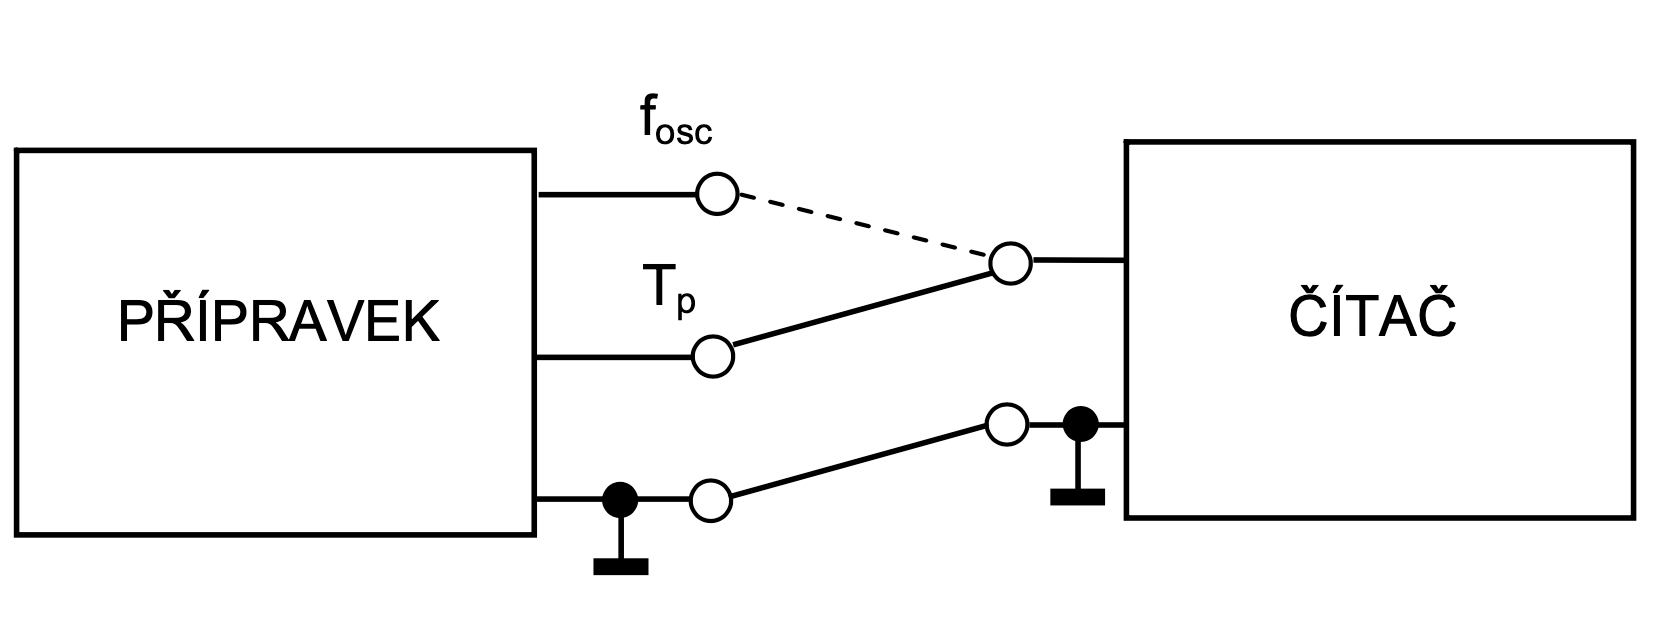
\includegraphics[width=.6\textwidth]{schema.png}
  \caption{Schéma zapojení měření na přípravku}
  \label{fig:schema}
\end{figure}

\section{Seznam použitých přístrojů}
\begin{table}[h!]
  \begin{tabular}{ll}
    GENERÁTOR &- nízkofrekvenční generátor, typ GOLDSTAR FG-8002\\
    ČÍTAČ &- univerzální čítač, typ \textit{made by ČVUT}\\
    PŘÍPRAVEK &- přípravek s hodinami řízenými krystalem\\
  \end{tabular}
\end{table}
\section{Teoretický úvod}
Měření frekvence a~doby periody je zpravidla provázeno čítačem. Ten v~závislosti na nastaveném typu měření měří následovně. Při měření frekvence ve vstupní signál upraven podle blokového schéma~\ref{schema:frce}. Signál prochází zesílením a~tvarovačem, díky čemuž se stane vhodným pro hradlo. Toto hradlo počítá kmity za danou periodu. Ta je dána vnitřním krystalovým oscilátorem.

Pro měření doby periody naopak použijeme zapojení podle schématu \ref{schema:perioda}. V tomto režimu vstupním signálem určujeme, jak dlouho bude hradlo otevřeno, zatímco mu z krystalového oscilátoru sypeme kmity, dokud to jde. Podle kmitů, které se vešly do doby jedné periody vstupního signálu poté určíme dobu periody.
\begin{schema}[h!]
  \centering
  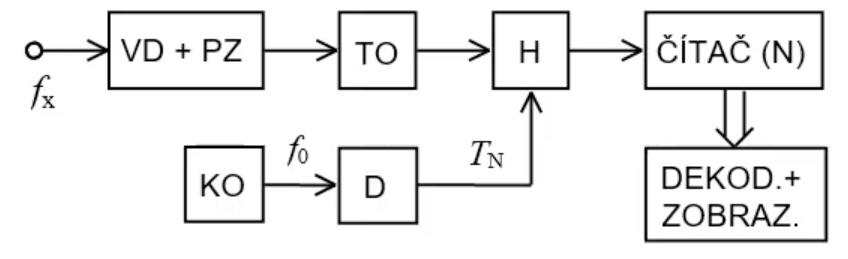
\includegraphics[width=.6\textwidth]{frce.png}
  \caption{Režim měření frekvence}
  \label{schema:frce}
\end{schema}

\begin{schema}[h!]
  \centering
  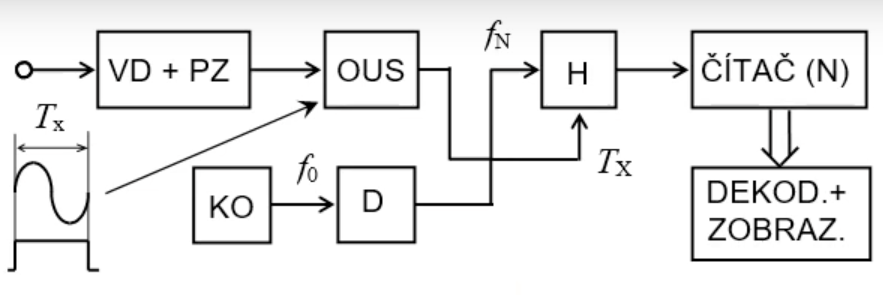
\includegraphics[width=.6\textwidth]{perioda.png}
  \caption{Režim měření doby periody}
  \label{schema:perioda}
\end{schema}


\section{Naměřené hodnoty}
Naměřená data z měření frekvenčního generátoru jsou v~tabulce~\ref{tab:frce} a~\ref{tab:perioda}.

\begin{table}[h!]
  \centering
  \begin{tabular}{|r|r|r|r|}
    \hline
      &60 Hz [Hz]&10 kHz [kHz]&100 kHz [kHz]\\\hline\hline
    0,1 s&70&10,63&110,83\\\hline
    1 s&68&10,622&110,828\\\hline
    10 s&67,9&10,6231&110,8373\\\hline
  \end{tabular}
  \label{tab:frce}
  \caption{Naměřené hodnoty frekvence}
\end{table}

\begin{table}[h!]
  \centering
  \begin{tabular}{|r|r|r|r|}
    \hline
    &60 Hz [\tmu s]&10 kHz [\tmu s]&100 kHz [\tmu s]\\\hline\hline
    1 T&15100,7&93,6&9\\\hline
    10 T &15101,87&93,64&-\\\hline
    100 T&-&93,6488&-\\\hline
    1000 T&-&93,63633&9,05553\\\hline
  \end{tabular}
  \label{tab:perioda}
  \caption{Naměřené hodnoty periody}
\end{table}

Data z měření hodin jsou v~tabulce~\ref{tab:hodiny}.

\begin{table}
  \centering
  \begin{tabular}{|c|c|}
    \hline
    f [kHz]&T [\tmu s]\\\hline\hline
    32,7677&2000038,9\\\hline
  \end{tabular}
  \caption{Hodnoty pro ručičkové hodiny}
  \label{tab:hodiny}
\end{table}




\section{Zpracování naměřených hodnot}
Pro určení nejistoty měření frekvence způsobenou rozlišením budeme vycházet ze vzorce \ref{eq:nejistota_frce}.

\begin{equation}
  u_{f_X} = \sqrt{\left(\Delta'f_X/\sqrt{3}\right)^2+\left(\Delta f_X/\sqrt{3}\right)^2}
  \label{eq:nejistota_frce}
\end{equation}

\begin{table}
  \centering
  \begin{tabular}{|c|c|c|c|}
    \hline
    &60 Hz [Hz]&10 kHz [Hz]&100 kHz [Hz]\\\hline\hline
    0,1&5,773502692&5,773502822&5,773516875\\\hline
    1&0,577350269&0,577351572&0,577492082\\\hline
    10&0,057735027&0,057748056&0,059136555\\\hline
  \end{tabular}
  \caption{Nejistoty měření frekvence}
\end{table}

Pro určení nejistoty měření doby periody způsobenou rozlišením budeme vycházet ze vzorce \ref{eq:nejistota_perioda}.

\begin{equation}
  u_{T_X} = \sqrt{\left(\Delta'T_X/\sqrt{3}\right)^2+\left(\Delta T_X/\sqrt{3}\right)^2+2u_k^2}
  \label{eq:nejistota_perioda}
\end{equation}

Jelikož neznáme efektivní hodnotu šumu vstupního zesilovače, nemůžeme určit člen $u_k^2$ a~budeme ho proto ignorovat. Nejistoty jsou dále v~tabulce.

\begin{table}[h!]
  \centering
  \begin{tabular}{|c|c|c|c|}
    \hline
    T, T= 1 \tmu s&60 Hz [\tmu s]&10 kHz [\tmu s]&100 kHz [\tmu s]\\\hline\hline
    1&0,001743679&1,08234E-05&1,18884E-06\\\hline
    10&0,001743823&1,22575E-05&\\\hline
    100&&5,8739E-05&\\\hline
    1000&&0,000577452&0,000577351\\\hline
  \end{tabular}
  \caption{Nejistoty měření periody}
\end{table}

Pro zjištění přesnosti hodin použijeme rovnice \ref{eq:presnost_T} a~\ref{eq:presnost_f}. Budeme vycházet z toho, že den má $24\cdot 60\cdot 60 = 86\,400~s$. 

\begin{equation}
  \left(\frac{T_m}{T}-1\right)\cdot 86\,400~s = \left(\frac{2,0000389}{2}-1\right)\cdot 86\,400~s = 1,68~\textrm{s/den}
  \label{eq:presnost_T}
\end{equation}

\begin{equation}
  \left(\frac{f_m}{f}-1\right)\cdot 86\,400~s = \left(\frac{32\,767,7}{32\,768}-1\right)\cdot 86\,400~s~=~-0,79~\textrm{s/den}
  \label{eq:presnost_f}
\end{equation}

Relativní chyba stupnice vůči měřené hodnotě je zobrazena v~tabulce níže.

\begin{table}[h!]
  \centering
  \begin{tabular}{|c|c|c|c|}
    \hline
    &60 Hz [Hz]&10 kHz [Hz]&100 kHz [Hz]\\\hline\hline
    Naměřeno&67,9&10623,1&110837,3\\\hline
    Absolutní chyba&7,9&623,1&10837,3\\\hline\hline
    Relativní chyba&0,12&0,059&0,098\\\hline
  \end{tabular}
  \label{tab:chyba}
  \caption{Relativní chyba stupnice na generátoru funkcí}
\end{table}

\section{Závěrečné vyhodnocení}
Zjistili jsme nepřesnost hodin a~jaký rozchod můžeme čekat za den. Také jsme ověřili, jak se při průměrování a~při používání delšího časového okna pro počítání tiků může zvýšit přesnost resp. snížit nejistota měření. Dále jsme zjistili absolutní a~relativní chybu stupnice generátoru funkcí. Zjistili jsme, že právě nastavení frekvence byl největší zdroj chyby.

%--- LITERATURA a~ZDROJE (povinne) ---
\clearpage
\renewcommand{\refname}{Seznam použité literatury a~zdrojů informací} 
%\section*{Seznam použité literatury a~zdrojů informací}
\phantomsection %pridej odkaz do PDF zalozek
\addcontentsline{toc}{section}{Seznam použité literatury a~zdrojů informací}

\begin{thebibliography}{99}

%----------------------------------------------------
\subsection*{Seznam použitých internetových zdrojů}
    \bibitem{navod} Návod k~laboratorní úloze
    
\end{thebibliography}

\end{document}